\begin{frame}{Executive summary}

\begin{itemize}
\itemsep1pt\parskip0pt\parsep0pt
\item
  16p11.2 deletion carriers exhibited delalyed M100 latencies\\
\item
  Differences are larger than in `idiopathic' ASD\\
\item
  No oberserved differences between controls and 16p11.2 duplication
  carriers
\end{itemize}

\end{frame}

\begin{frame}{Participants (recruited)}

\begin{itemize}
\itemsep1pt\parskip0pt\parsep0pt
\item
  137 children\\
\item
  CHOP: 63, UCSF: 74
\item
  46 16p11.2 deletion carriers\\
\item
  26 16p11.2 duplication carriers\\
\item
  66 age-matched controls
\end{itemize}

\end{frame}

\begin{frame}{Participants (final)}

\begin{itemize}
\itemsep1pt\parskip0pt\parsep0pt
\item
  99 children\\
\item
  CHOP: 47, UCSF: 52\\
\item
  35 16p11.2 deletion carriers\\
\item
  16 16p11.2 duplication carriers\\
\item
  48 age-matched controls
\end{itemize}

\end{frame}

\begin{frame}{Particpants (final)}

\begin{longtable}[c]{@{}llll@{}}
\toprule
--- & Controls & Deletions & Duplications\tabularnewline
\midrule
\endhead
Age range (years) & 7.31 - 17.15 & 7.98 - 17.03 & 7.38 -
16.92\tabularnewline
Mean age (years) & 12.82±2.56 & 11.32±.2.65 & 11.45±2.41\tabularnewline
N (evaluable) & 45 & 35 & 16\tabularnewline
NVIQ & 105.73±11.88 & 90.09±15.07 & 83.06±10.68\tabularnewline
VIQ & 107.24±13.72 & 85.37±17.05 & 91.69±14.09\tabularnewline
CELF-4 & 106.22±11.22 & 75.81±20.80 & 84.62±13.18\tabularnewline
SRS & 16.68±11.89 & 71.51±34.38 & 72.06±41.22\tabularnewline
CTOPP & 9.23±1.95 & 5.64±2.64 & 7.64±1.45\tabularnewline
\bottomrule
\end{longtable}

\end{frame}

\begin{frame}{Procedure}

\begin{itemize}
\itemsep1pt\parskip0pt\parsep0pt
\item
  passive presentation of binaural sinusoidal tones\\
\item
  recording from whole-head magnetometer\\
\item
  analysis: artifact rejection, bandpass filtering, source estimation
\end{itemize}

\end{frame}

\begin{frame}{Statistical analysis}

\begin{itemize}
\itemsep1pt\parskip0pt\parsep0pt
\item
  M100 latency: dependent variable\\
\item
  Linear Mixed Models via \texttt{lme4}\\
\item
  model:
  \texttt{Hemisphere\ +\ Stimulus\ Condition\ +\ Case\ +\ Age\ +\ Site\ +\ (Stimulus\ Condition\ +\ Hemisphere\ \textbar{}\ Subject)}\\
\item
  significance: Wald Type II \(\chi\)\textsuperscript{2} tests; Tukey
  HSD, correlation tests
\end{itemize}

\end{frame}

\begin{frame}{Complete observations}

\begin{longtable}[c]{@{}lrrr@{}}
\toprule
Case & compCases & n & failCases\tabularnewline
\midrule
\endhead
control & 266 & 384 & 118\tabularnewline
deletion & 203 & 280 & 77\tabularnewline
duplication & 65 & 128 & 63\tabularnewline
\bottomrule
\end{longtable}

\end{frame}

\begin{frame}{M100 latency effects - condition means}

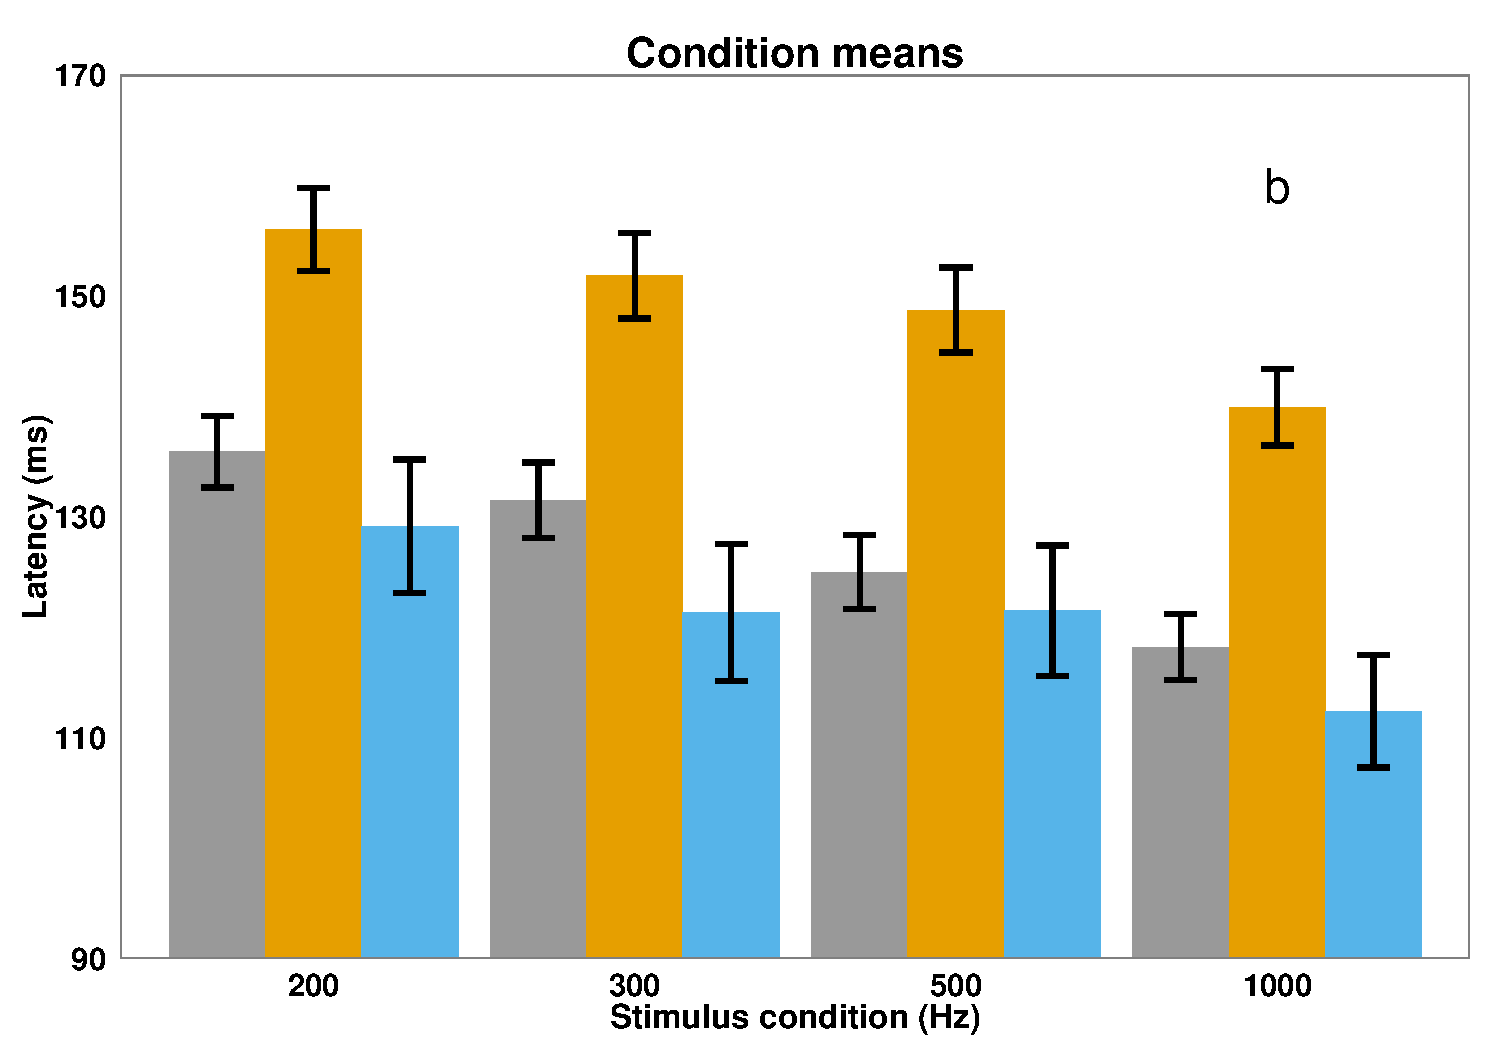
\includegraphics{m100-beamer-presentation-version_files/figure-beamer/condition means-1.pdf}

\end{frame}

\begin{frame}{M100 latency effects - hemisphere means}

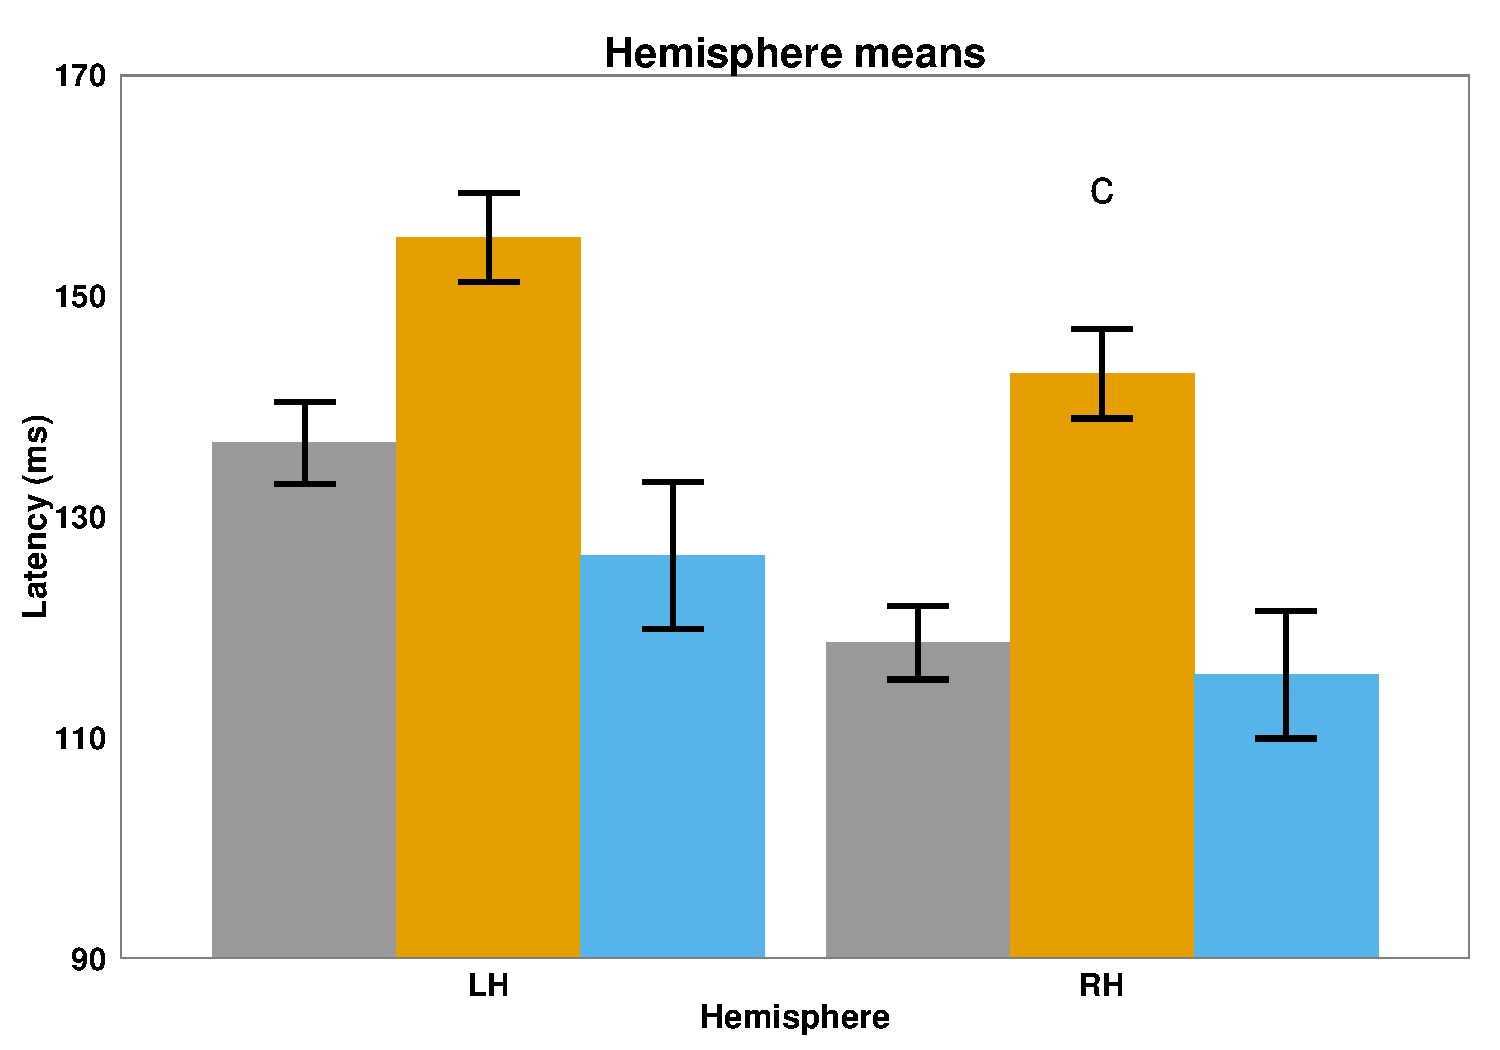
\includegraphics{m100-beamer-presentation-version_files/figure-beamer/hemisphere means-1.pdf}

\end{frame}

\begin{frame}{M100 latency effects - mean responses}

\begin{longtable}[c]{@{}llll@{}}
\toprule
Mean & Controls & Deletions & Duplications\tabularnewline
\midrule
\endhead
Overall (ms) & 127.2±3.1 & 149.0±3.6 & 120.9±5.3\tabularnewline
LH (ms) & 136.7±3.7 & 155.3±4.0 & 126.5±6.6\tabularnewline
RH (ms) & 118.6±3.3 & 143.0±4.1 & 115.7±5.8\tabularnewline
\bottomrule
\end{longtable}

\end{frame}

\begin{frame}{Effect size estimation}

\begin{longtable}[c]{@{}lrrrrr@{}}
\toprule
lhs & rhs & estimate & se & t & p\tabularnewline
\midrule
\endhead
deletion - control & 0 & 20.9 & 4.3 & 4.8 & 0.0\tabularnewline
duplication - control & 0 & -5.4 & 5.6 & -1.0 & 0.6\tabularnewline
duplication - deletion & 0 & -26.4 & 5.6 & -4.7 & 0.0\tabularnewline
\bottomrule
\end{longtable}

\end{frame}

\begin{frame}{Variance differences}

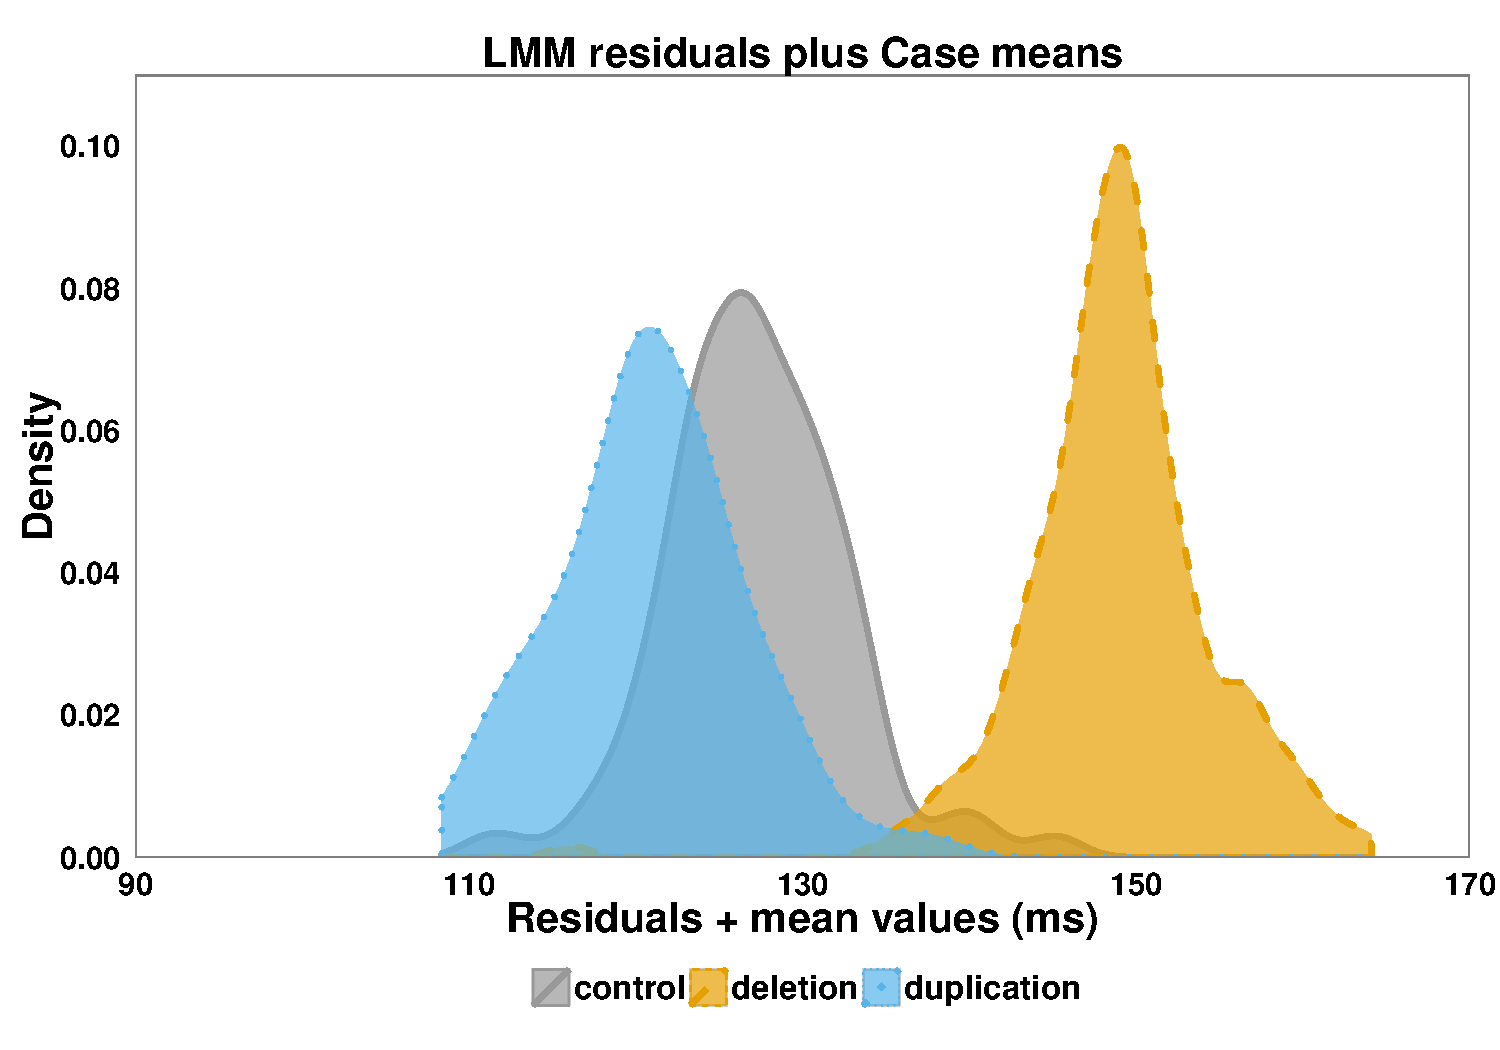
\includegraphics{m100-beamer-presentation-version_files/figure-beamer/residuals plus means-1.pdf}

\end{frame}

\begin{frame}{Conclusion}

\begin{itemize}
\itemsep1pt\parskip0pt\parsep0pt
\item
  main result: \textasciitilde{}20 ms delay in M100 component in 16p11.2
  deletion carriers\\
\item
  no observed significant difference bewtween 16p11.2 duplication
  carriers and controls\\
\item
  effects not inconsistent with other reported effects
\item
  support for gene-neurophysiology association
\end{itemize}

\end{frame}
